\documentclass{standalone}
\usepackage{tikz}
\usetikzlibrary{patterns}
\usetikzlibrary{positioning}
\usetikzlibrary{patterns, positioning}
\usetikzlibrary{shapes.misc}
\usepackage[outline]{contour}
\contourlength{1.5pt} 
\usepackage[sfdefault]{ClearSans}

\begin{document}
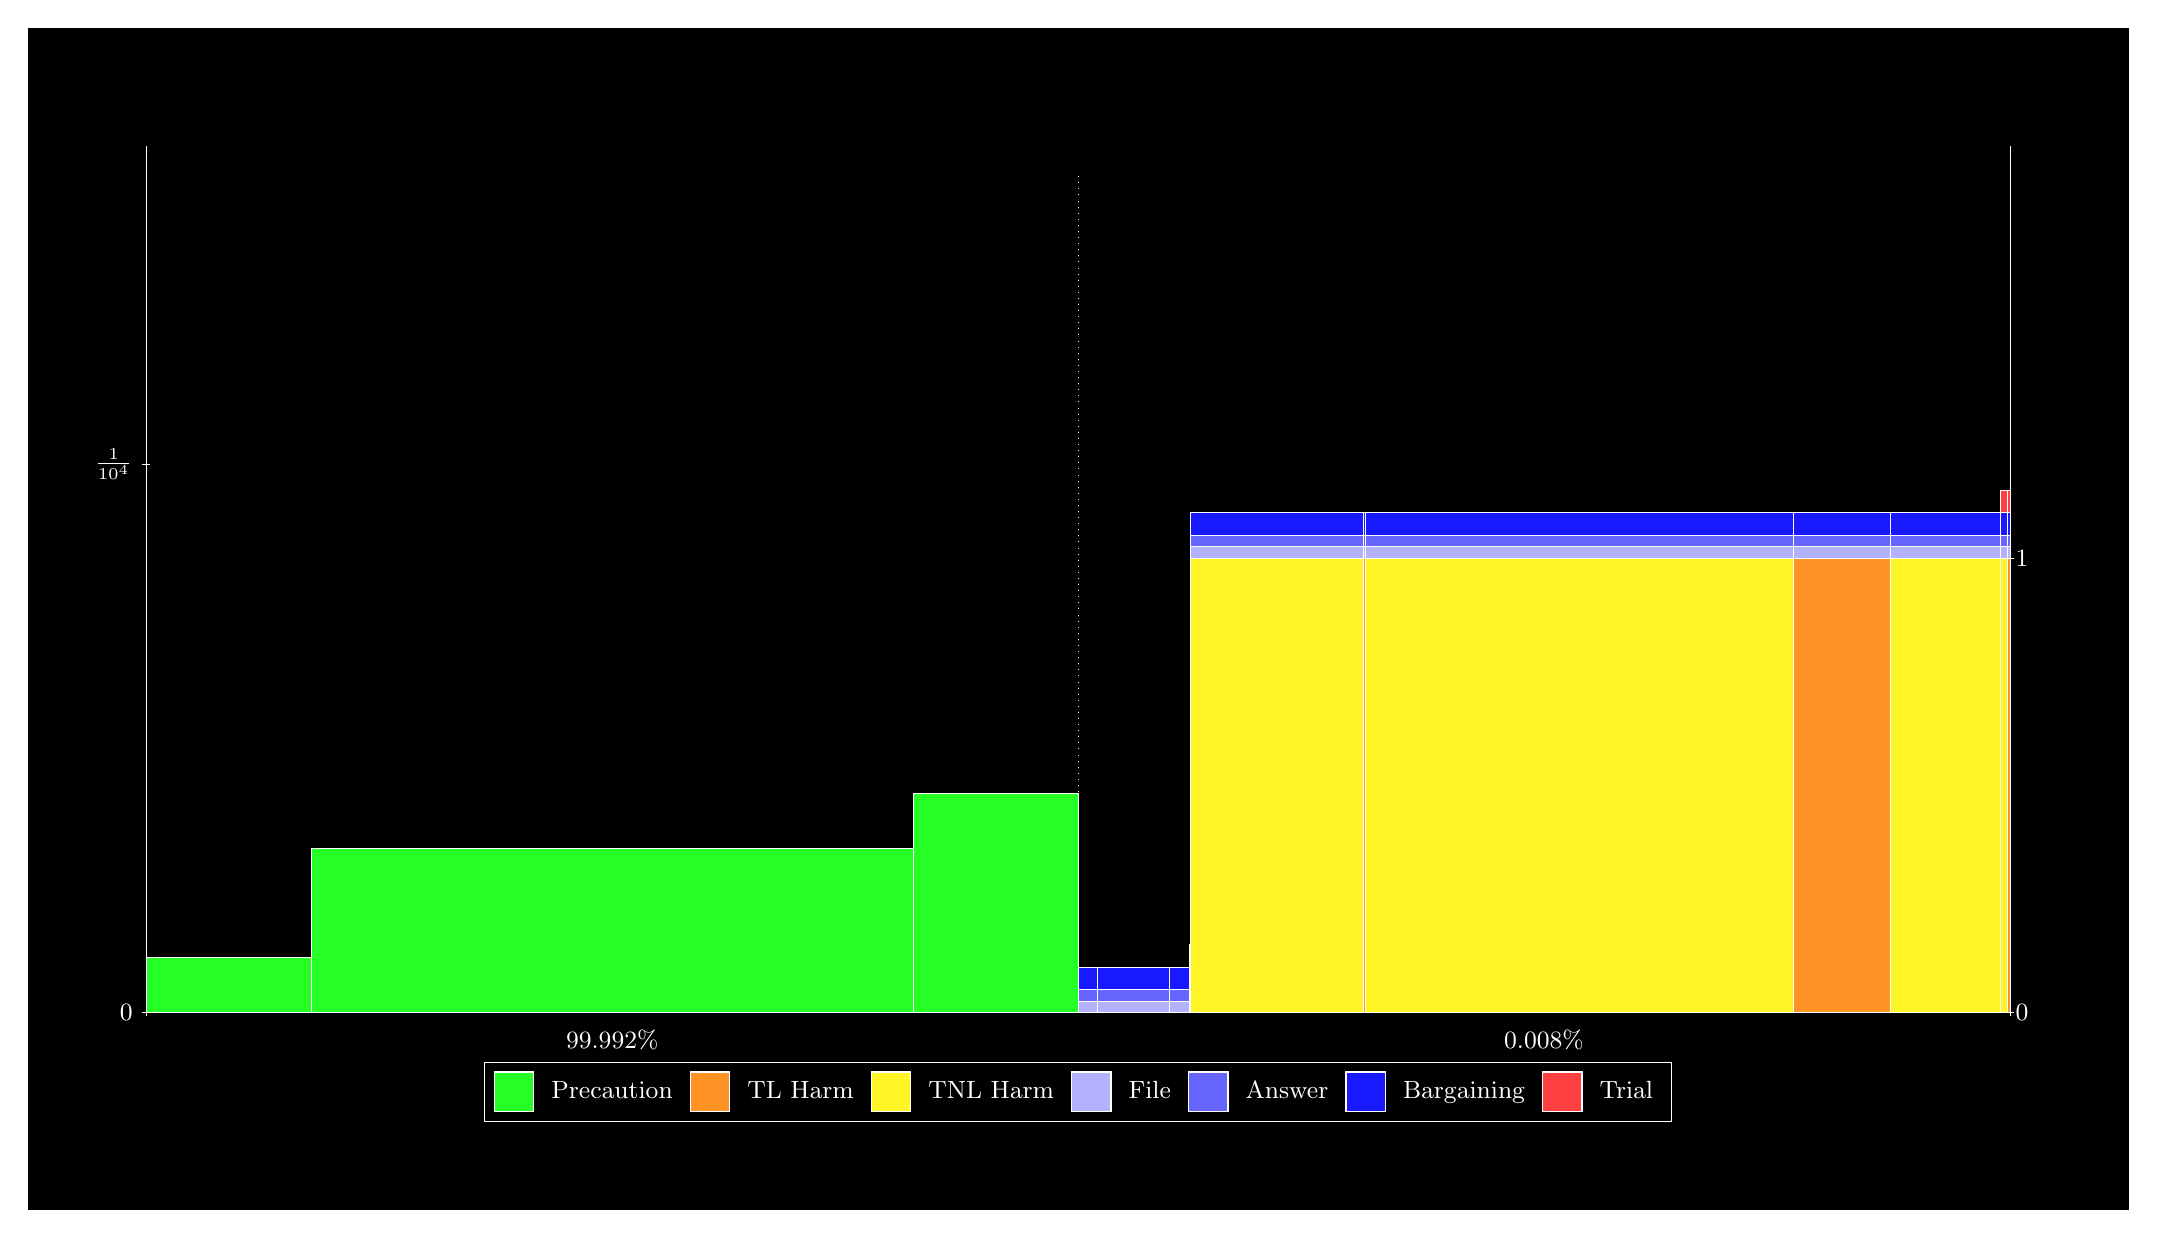
\begin{tikzpicture}
\draw[fill=black] (0,0) rectangle (26.667,15);
\draw[fill=green!85,draw=white,very thin] (1.5,2.5) rectangle (3.5989,3.1963);
\draw[fill=green!85,draw=white,very thin] (3.5989,2.5) rectangle (11.234,4.5888);
\draw[fill=green!85,draw=white,very thin] (11.234,2.5) rectangle (13.333,5.2851);
\draw[fill=green!85,draw=white,very thin] (13.333,2.5) rectangle (13.573,2.5001);
\draw[fill=blue!30,draw=white,very thin] (13.333,2.5001) rectangle (13.573,2.6443);
\draw[fill=blue!60,draw=white,very thin] (13.333,2.6443) rectangle (13.573,2.7886);
\draw[fill=blue!90,draw=white,very thin] (13.333,2.7886) rectangle (13.573,3.0772);
\draw[fill=green!85,draw=white,very thin] (13.573,2.5) rectangle (14.494,2.5002);
\draw[fill=blue!30,draw=white,very thin] (13.573,2.5002) rectangle (14.494,2.6445);
\draw[fill=blue!60,draw=white,very thin] (13.573,2.6445) rectangle (14.494,2.7887);
\draw[fill=blue!90,draw=white,very thin] (13.573,2.7887) rectangle (14.494,3.0773);
\draw[fill=green!85,draw=white,very thin] (14.494,2.5) rectangle (14.748,2.5002);
\draw[fill=blue!30,draw=white,very thin] (14.494,2.5002) rectangle (14.748,2.6445);
\draw[fill=blue!60,draw=white,very thin] (14.494,2.6445) rectangle (14.748,2.7888);
\draw[fill=blue!90,draw=white,very thin] (14.494,2.7888) rectangle (14.748,3.0774);
\draw[fill=green!85,draw=white,very thin] (14.748,2.5) rectangle (14.761,2.5001);
\draw[fill=blue!30,draw=white,very thin] (14.748,2.5001) rectangle (14.761,2.6443);
\draw[fill=blue!60,draw=white,very thin] (14.748,2.6443) rectangle (14.761,2.7886);
\draw[fill=blue!90,draw=white,very thin] (14.748,2.7886) rectangle (14.761,3.0772);
\draw[fill=red!75,draw=white,very thin] (14.748,3.0772) rectangle (14.761,3.3658);
\draw[fill=green!85,draw=white,very thin] (14.761,2.5) rectangle (16.957,2.5001);
\draw[fill=yellow!85,draw=white,very thin] (14.761,2.5001) rectangle (16.957,8.2714);
\draw[fill=blue!30,draw=white,very thin] (14.761,8.2714) rectangle (16.957,8.4156);
\draw[fill=blue!60,draw=white,very thin] (14.761,8.4156) rectangle (16.957,8.5599);
\draw[fill=blue!90,draw=white,very thin] (14.761,8.5599) rectangle (16.957,8.8485);
\draw[fill=green!85,draw=white,very thin] (16.957,2.5) rectangle (16.986,2.5001);
\draw[fill=orange!85,draw=white,very thin] (16.957,2.5001) rectangle (16.986,8.2714);
\draw[fill=blue!30,draw=white,very thin] (16.957,8.2714) rectangle (16.986,8.4156);
\draw[fill=blue!60,draw=white,very thin] (16.957,8.4156) rectangle (16.986,8.5599);
\draw[fill=blue!90,draw=white,very thin] (16.957,8.5599) rectangle (16.986,8.8485);
\draw[fill=green!85,draw=white,very thin] (16.986,2.5) rectangle (22.418,2.5002);
\draw[fill=yellow!85,draw=white,very thin] (16.986,2.5002) rectangle (22.418,8.2715);
\draw[fill=blue!30,draw=white,very thin] (16.986,8.2715) rectangle (22.418,8.4157);
\draw[fill=blue!60,draw=white,very thin] (16.986,8.4157) rectangle (22.418,8.56);
\draw[fill=blue!90,draw=white,very thin] (16.986,8.56) rectangle (22.418,8.8486);
\draw[fill=green!85,draw=white,very thin] (22.418,2.5) rectangle (23.647,2.5002);
\draw[fill=orange!85,draw=white,very thin] (22.418,2.5002) rectangle (23.647,8.2715);
\draw[fill=blue!30,draw=white,very thin] (22.418,8.2715) rectangle (23.647,8.4157);
\draw[fill=blue!60,draw=white,very thin] (22.418,8.4157) rectangle (23.647,8.56);
\draw[fill=blue!90,draw=white,very thin] (22.418,8.56) rectangle (23.647,8.8486);
\draw[fill=green!85,draw=white,very thin] (23.647,2.5) rectangle (25.046,2.5002);
\draw[fill=yellow!85,draw=white,very thin] (23.647,2.5002) rectangle (25.046,8.2715);
\draw[fill=blue!30,draw=white,very thin] (23.647,8.2715) rectangle (25.046,8.4158);
\draw[fill=blue!60,draw=white,very thin] (23.647,8.4158) rectangle (25.046,8.5601);
\draw[fill=blue!90,draw=white,very thin] (23.647,8.5601) rectangle (25.046,8.8487);
\draw[fill=green!85,draw=white,very thin] (25.046,2.5) rectangle (25.135,2.5001);
\draw[fill=yellow!85,draw=white,very thin] (25.046,2.5001) rectangle (25.135,8.2714);
\draw[fill=blue!30,draw=white,very thin] (25.046,8.2714) rectangle (25.135,8.4156);
\draw[fill=blue!60,draw=white,very thin] (25.046,8.4156) rectangle (25.135,8.5599);
\draw[fill=blue!90,draw=white,very thin] (25.046,8.5599) rectangle (25.135,8.8485);
\draw[fill=red!75,draw=white,very thin] (25.046,8.8485) rectangle (25.135,9.137);
\draw[fill=green!85,draw=white,very thin] (25.135,2.5) rectangle (25.167,2.5001);
\draw[fill=orange!85,draw=white,very thin] (25.135,2.5001) rectangle (25.167,8.2714);
\draw[fill=blue!30,draw=white,very thin] (25.135,8.2714) rectangle (25.167,8.4156);
\draw[fill=blue!60,draw=white,very thin] (25.135,8.4156) rectangle (25.167,8.5599);
\draw[fill=blue!90,draw=white,very thin] (25.135,8.5599) rectangle (25.167,8.8485);
\draw[fill=red!75,draw=white,very thin] (25.135,8.8485) rectangle (25.167,9.137);
\draw[white,very thin] (1.5,2.5) -- (1.5,13.5);
\draw[white,very thin] (1.45,2.5) -- (1.55,2.5);
\node[font=\small,text=white, anchor=east] at (1.45, 2.5) {0};
\draw[white,very thin] (1.45,9.4628) -- (1.55,9.4628);
\node[font=\small,text=white, anchor=east] at (1.45, 9.4628) {$\frac{1}{10^{4}}$};

\draw[white,dotted,very thin] (13.333,2.83) -- (13.333,13.17);
\draw[white,very thin] (25.167,2.5) -- (25.167,13.5);
\draw[white,very thin] (25.117,2.5) -- (25.217,2.5);
\node[font=\small,text=white, anchor=west] at (25.117, 2.5) {0};
\draw[white,very thin] (25.117,8.2713) -- (25.217,8.2713);
\node[font=\small,text=white, anchor=west] at (25.117, 8.2713) {1};

\draw[white,very thin] (1.5,2.5) -- (25.167,2.5);
\draw[white,very thin] (1.5,2.45) -- (1.5,2.55);
\node[font=\small,text=white, anchor=north] at (1.5, 2.45) {};
\draw[white,very thin] (25.167,2.45) -- (25.167,2.55);
\node[font=\small,text=white, anchor=north] at (25.167, 2.45) {};

\node[font=\small,text=white,anchor=south] at (7.4167, 1.9) {99.992\%};
\node[font=\small,text=white,anchor=south] at (19.25, 1.9) {0.008\%};
\draw (13.3333,2.5) node (B) {};
\begin{scope}[align=center]
\matrix[scale=0.5,draw=white,below=0.5cm of B,nodes={draw},column sep=0.1cm]{
\node[rectangle,draw,minimum width=0.5cm,minimum height=0.5cm,fill=green!85]{}; & \node[draw=none,font=\small,text=white]{Precaution}; &
\node[rectangle,draw,minimum width=0.5cm,minimum height=0.5cm,fill=orange!85]{}; & \node[draw=none,font=\small,text=white]{TL Harm}; &
\node[rectangle,draw,minimum width=0.5cm,minimum height=0.5cm,fill=yellow!85]{}; & \node[draw=none,font=\small,text=white]{TNL Harm}; &
\node[rectangle,draw,minimum width=0.5cm,minimum height=0.5cm,fill=blue!30]{}; & \node[draw=none,font=\small,text=white]{File}; &
\node[rectangle,draw,minimum width=0.5cm,minimum height=0.5cm,fill=blue!60]{}; & \node[draw=none,font=\small,text=white]{Answer}; &
\node[rectangle,draw,minimum width=0.5cm,minimum height=0.5cm,fill=blue!90]{}; & \node[draw=none,font=\small,text=white]{Bargaining}; &
\node[rectangle,draw,minimum width=0.5cm,minimum height=0.5cm,fill=red!75]{}; & \node[draw=none,font=\small,text=white]{Trial}; \\\\
};\end{scope}

\end{tikzpicture}
\end{document}